\mychapter{Análise Léxica}
\label{Cap:Léxico}

\section{Enunciado}
\begin{enumerate}

\item{Quais são as funções do analisador léxico nos compiladores/interpretadores?}

\item{Quais as vantagens e desvantagens da implementação do analisador léxico como uma fase separada do
processamento da linguagem de programação em relação à sua implementação como sub-rotina que vai
extraindo um átomo a cada chamada?}

\item{Defina formalmente, através de expressões regulares sobre o conjunto de caracteres ASCII, a sintaxe de cada um dos tipos de átomos a serem extraídos do texto-fonte pelo analisador léxico, bem como de cada um dos
espaçadores e comentários.}

\item{Converta cada uma das expressões regulares, assim obtidas, em autômatos finitos equivalentes que reconheçam as correspondentes linguagens por elas definidas.}

\item{Crie um autômato único que aceite todas essas linguagens a partir de um mesmo estado inicial, mas que apresente um estado final diferenciado para cada uma delas.}

\item{Transforme o autômato assim obtido em um transdutor, que emita como saída o átomo encontrado ao abandonar cada um dos estados finais para iniciar o reconhecimento de mais um átomo do texto.}

\item{Converta o transdutor assim obtido em uma sub-rotina, escrita na linguagem de programação de sua preferência. Não se esqueça que o final de cada átomo é determinado ao ser encontrado o primeiro símbolo do átomo ou do espaçador seguinte. Esse símbolo não pode ser perdido, devendo-se, portanto, tomar os cuidados de programação que forem necessários para reprocessá-los, apesar de já terem sido lidos pelo autômato.}

\item{Crie um programa principal que chame repetidamente a sub-rotina assim construída, e a aplique sobre um arquivo do tipo texto contendo o texto-fonte a ser analisado. Após cada chamada, esse programa principal deve imprimir as duas componentes do átomo extraído (o tipo e o valor do átomo encontrado). Faça o programa parar quando o programa principal receber do analisador léxico um átomo especial indicativo da ausência de novos átomos no texto de entrada.}

\item{Relate detalhadamente o funcionamento do analisador léxico assim construído, incluindo no relatório: descrição teórica do programa; descrição da sua estrutura; descrição de seu funcionamento; descrição dos testes realizados e das saídas obtidas.}

\item{Explique como enriquecer esse analisador léxico com um expansor de macros do tipo \#DEFINE, não paramétrico nem recursivo, as que permita a qualquer macro chamar outras macros, de forma não cíclica.}

\end{enumerate}

\section{Introdução}
O analisador léxico tem como função ler o arquivo que contém o código escrito na linguagem origem e transformar esse conjunto de caracteres em um conjunto de tokens que possuam um significado na linguagem escrita. As atividades principais nesta fase são: conversão numérica, à identificação de palavras reservadas e criação e manutenção de tabelas de símbolos da compilação.

\section{Subrotina}
A desvantagem do analisador léxico como uma subrotina é a necessidade do envio de mensagens por parte do analisador sintático para requisitar um novo átomo. Além disso é necessário tomar muito cuidado para não tornar o algoritmo do analisador léxico ineficiente. A vantagem da fase de análise léxica como uma subrotina é o aumento da rapidez no processo de compilação como um todo, pois o analisador léxico é dedicado à tarefa de reconhecimento léxico, enquanto o analisador sintático realiza as funções mais pesadas, chamando o analisador léxico somente quando necessário.

\section{Construção}

A seguir, é mostrado o processo de construção do Analisador Léxico.

\subsection{Expressões regulares}

\textbf{Legenda:}\\
\textbf{<qualquer>:} qualquer caracter que não se encaixa nos tipos de entrada definidos\\
\textbf{<nova linha>:} caracter lido como `\textbackslash n'

\subsubsection{Átomos}

Há 10 tipos diferentes de átomos, e cada um está representado abaixo com suas respectivas sintaxes na forma de expressões regulares.

\begin{enumerate}
	\item String: ``<qualquer>+''|`<qualquer>+'
    \item Operadores aritméticos: ( + | - | * | / )
    \item Operadores booleanos: ( \&\& | || | !)
    \item Número: ([0-9]+ | [0-9]+.[0-9]+)
    \item Comparadores: ( > | < | <= | >= | == | != )
    \item Palavras Reservadas: (begin | do | end | if | elsif | endif | while | endwhile | function | endfunction | int | char | bool | float | return | true | false | print | scan | switch | case | continue | endswitch)
    \item Identificadores: [a-zA-Z]+[a-zA-Z0-9\_]+
    \item Separadores: ( [ | ] | \( | \) | , )
    \item Final de comando: (;)
    \item Desconhecido: <nenhuma das anteriores>    
    \item Atribuição: (=)
\end{enumerate}

\subsubsection{Não-átomos}

As sintaxes de elementos como comentários (de linha e de bloco) não fazem parte do conjunto de tipos de átomos pois devem ser ignorados durante a análise léxica. Entretanto, eles devem ser implementados no transdutor do analisador léxico, ortanto, estes foram definidos como não-átomos, e as sintaxes estão representadas abaixo por expressões regulares:

\begin{description}
	\item[Comentário de linha:] \#<qualquer>*<nova linha>
    \item[Comentário de bloco:] \#\#<qualquer>*\#\#
\end{description}

\subsection{Autômatos Finitos}

As expressões regulares dos diferentes tipos de átomos, juntamente não-átomos foram representadas abaixo na forma de autômatos finitos :\\

\textbf{Legenda:}\\
\textbf{<dig>:} [0-9]\\
\textbf{<letra>:} [a-zA-Z]\\
\textbf{<qualquer exceto''>:} qualquer símbolo lido exceto ''\\
\textbf{<qualquer exceto'>:} qualquer símbolo lido exceto '\\
\textbf{<desconhecido>:} qualquer símbolo não descrito pelos autômatos\\

\subsubsection{String}
\begin{figure}[H]
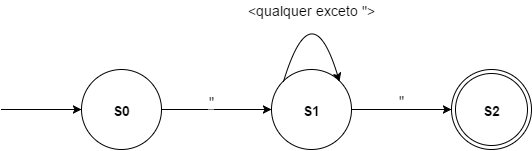
\includegraphics[width=10cm, keepaspectratio]{automatas/double_quotes.png}
\caption{\label{fig:double_quotes} Autômato: String com aspas duplas}
\end{figure}

\begin{figure}[H]
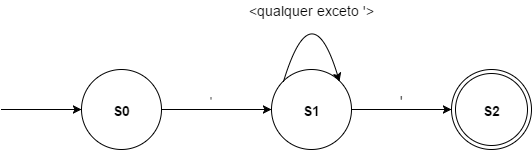
\includegraphics[width=10cm, keepaspectratio]{automatas/simple_quotes.png}
\caption{\label{fig:simple_quotes} Autômato: String com aspas simples}
\end{figure}

\subsubsection{Operadores aritméticos}
\begin{figure}[H]
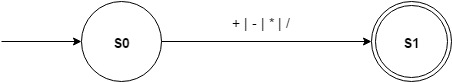
\includegraphics[width=8cm, keepaspectratio]{automatas/math_operators.png}
\caption{\label{fig:math_operators} Autômato: Operadores aritméticos}
\end{figure}

\subsubsection{Número}
\begin{figure}[H]
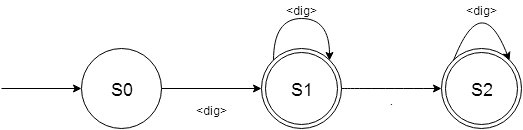
\includegraphics[width=10cm, keepaspectratio]{automatas/number.png}
\caption{\label{fig:number} Autômato: Número}
\end{figure}

\subsubsection{Atribuição}
\begin{figure}[H]
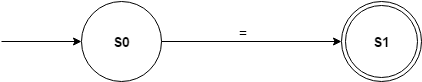
\includegraphics[width=8cm, keepaspectratio]{automatas/atribuicao.png}
\caption{\label{fig:assignment} Autômato: Atribuição}
\end{figure}

\subsubsection{Comparadores}
\begin{figure}[H]
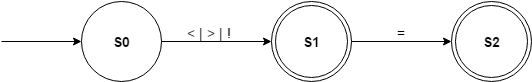
\includegraphics[width=10cm, keepaspectratio]{automatas/comparators.png}
\caption{\label{fig:comparators} Autômato: Comparadores}
\end{figure}

\subsubsection{Palavras reservadas}
\begin{figure}[H]
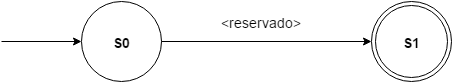
\includegraphics[width=8cm, keepaspectratio]{automatas/reserved.png}
\caption{\label{fig:reserved} Autômato: Palavras reservadas}
\end{figure}

\subsubsection{Identificadores}
\begin{figure}[H]
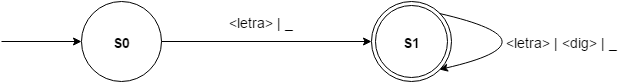
\includegraphics[width=10cm, keepaspectratio]{automatas/identifier.png}
\caption{\label{fig:identifiers} Autômato: Identificadores}
\end{figure}

\subsubsection{Separadores}
\begin{figure}[H]
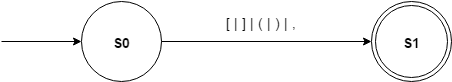
\includegraphics[width=8cm, keepaspectratio]{automatas/separators.png}
\caption{\label{fig:separators} Autômato: Separadores}
\end{figure}

\subsubsection{Final de comando}
\begin{figure}[H]
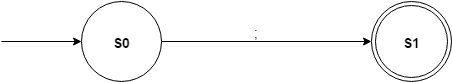
\includegraphics[width=8cm, keepaspectratio]{automatas/command_end.png}
\caption{\label{fig:command_end} Autômato: Final de comando}
\end{figure}

\subsubsection{Comentário de linha}
\begin{figure}[H]
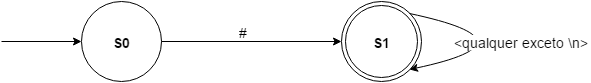
\includegraphics[width=10cm, keepaspectratio]{automatas/simple_comment.png}
\caption{\label{fig:simple_comment} Autômato: Comentário de linha}
\end{figure}

\subsubsection{Comentário de bloco}
\begin{figure}[H]
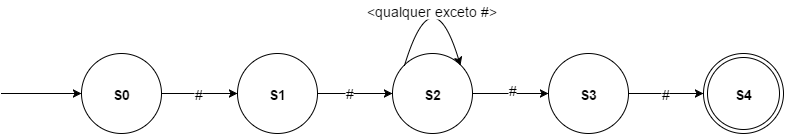
\includegraphics[width=13cm, keepaspectratio]{automatas/block_comment.png}
\caption{\label{fig:block_comment} Autômato: Comentário de bloco}
\end{figure}

\subsubsection{Desconhecido}
\begin{figure}[H]
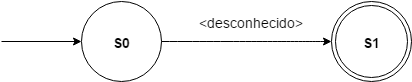
\includegraphics[width=8cm, keepaspectratio]{automatas/unknown.png}
\caption{\label{fig:unknown} Autômato: Desconhecido}
\end{figure}

Ao unificar os autômatos acima, tem-se um autômato que aceita todas as linguagens por elas definidas:

\subsubsection{Autômato unificado}
\begin{figure}[H]
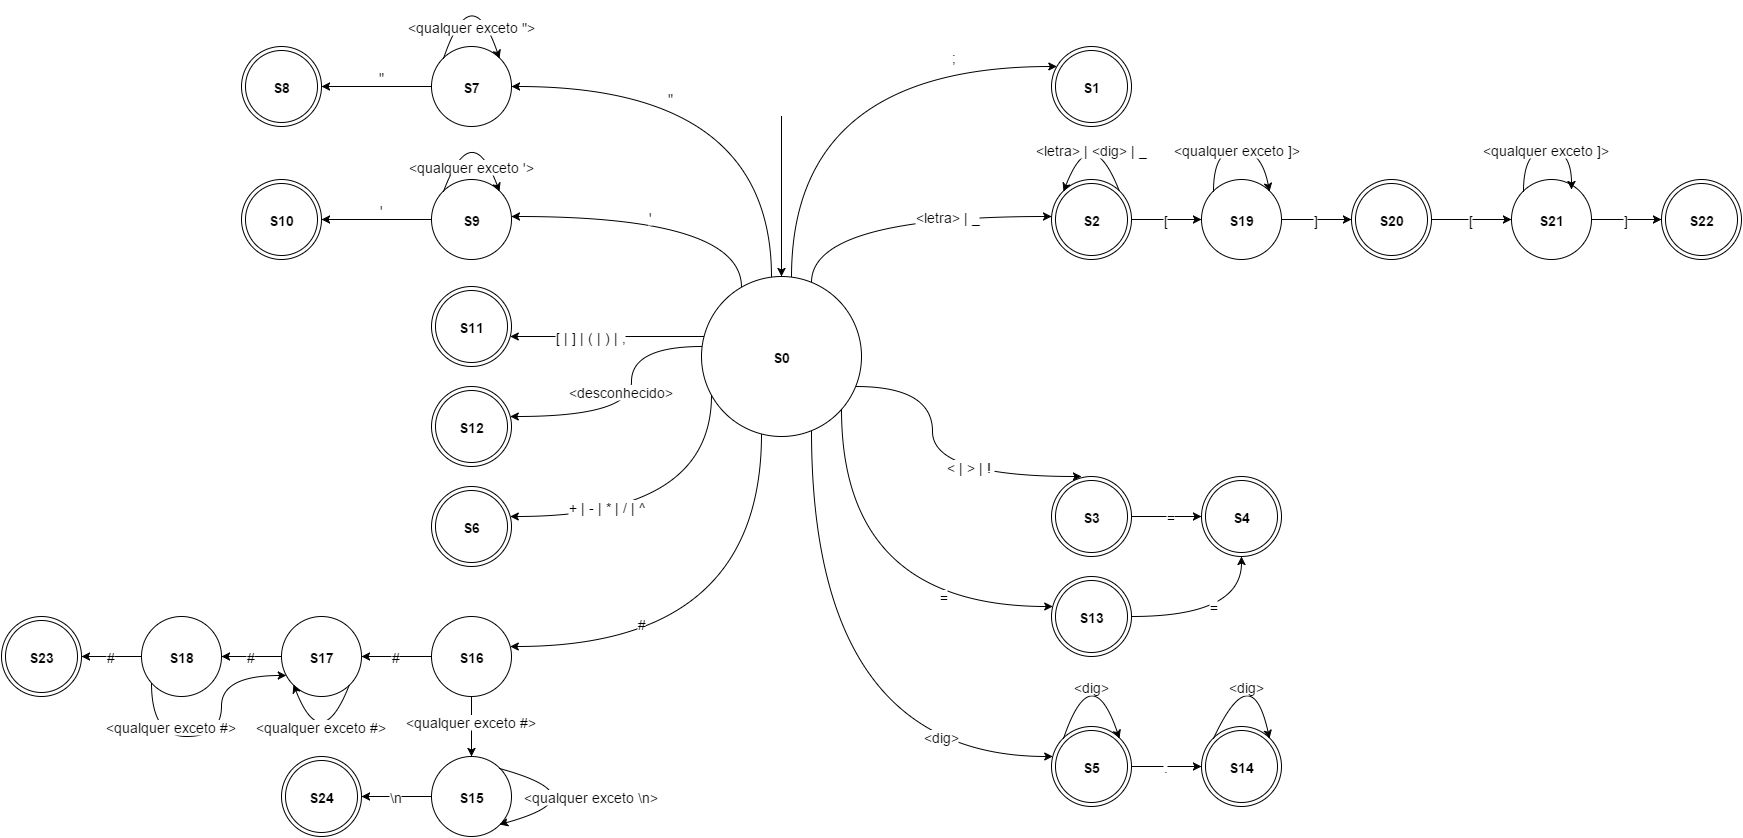
\includegraphics[width=1\textwidth]{automatas/unificado.png}
\caption{\label{fig:unified} Autômato: unificado}
\end{figure}

Através do autômato unificado pode-se representar o transdutor, que emite como saída o átomo ao sair dos estados finais para iniciar o reconhecimento de mais um átomo do texto.

\subsubsection{Transdutor}
\begin{figure}[H]
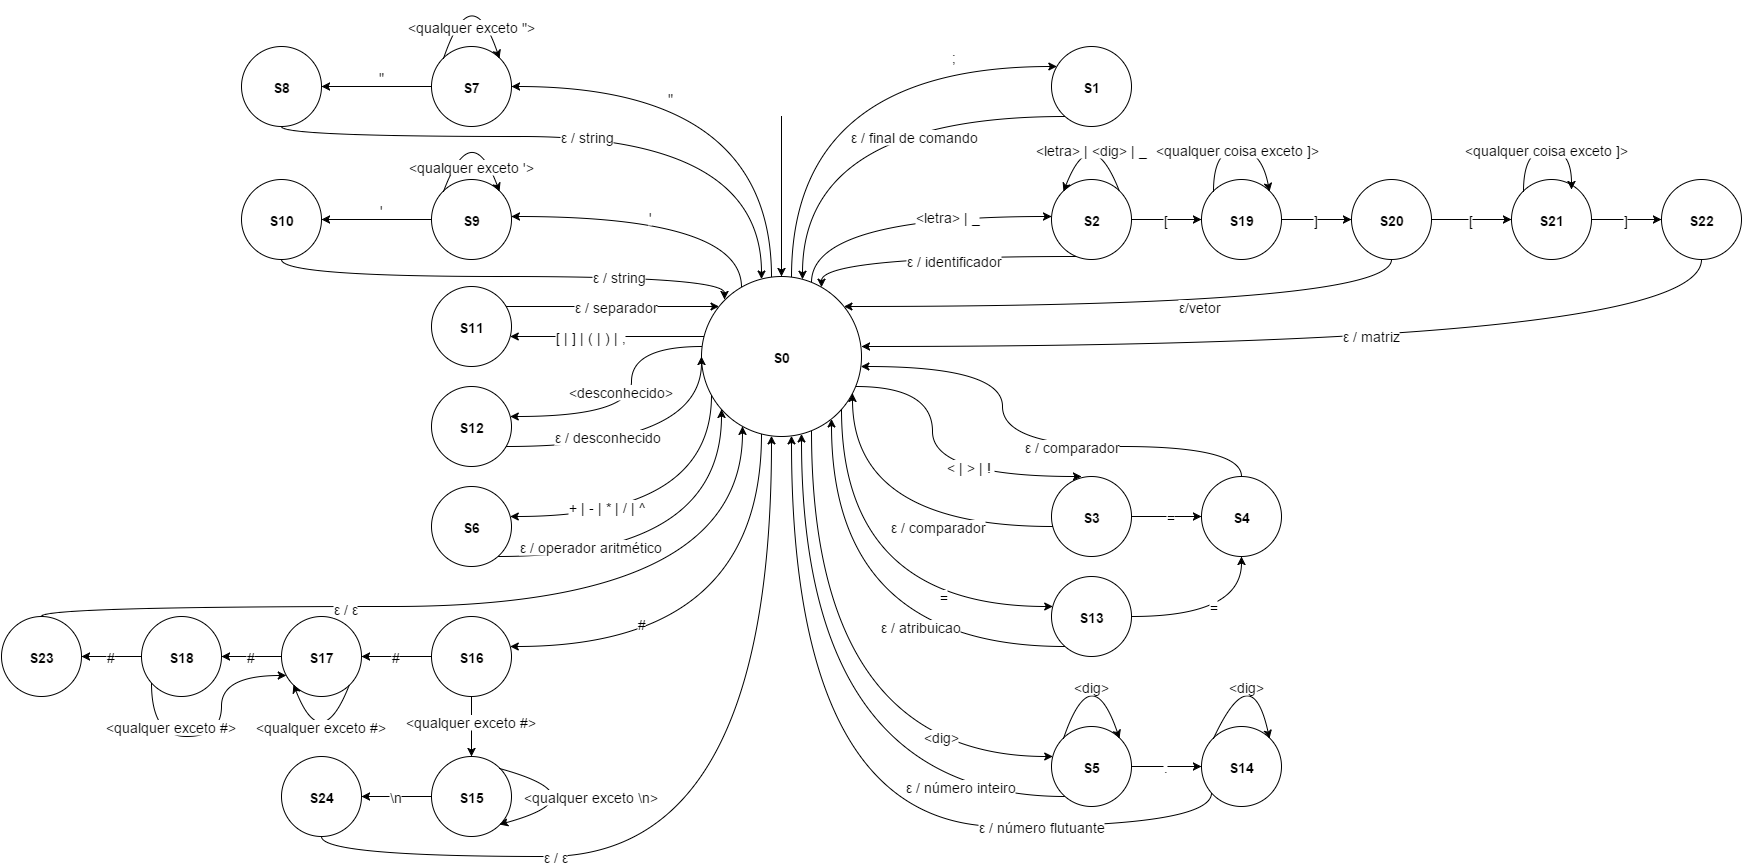
\includegraphics[width=1\textwidth]{automatas/transdutor.png}
\caption{\label{fig:transdutor} Autômato: Transdutor}
\end{figure}

\section{Estrutura do código}

Para a análise léxica foram usados alguns componentes programados:
\begin{itemize}
\item{token}
\item{transition\_table}
\item{automata}
\item{analisador}
\end{itemize}

\subsection{Token}
Arquivos: /utils/token.h e /utils/token.c\\
Auto explicativo, é uma estrutura que representa um token e guarda tanto o valor do token em characteres e o tipo do token, que se confundem com os dez tipos de linguagens obtidas em uma seção anterior.

\subsection{Transition table}
Arquivos: /transition\_table.h e /transition\_table.c\\
Contém a tabela de transição do transdutor (estado x tipo de entrada) e mais algumas funções auxiliares como um conversor de character para o tipo de entrada correspondente, a definição dos possíveis estados e os tipos de entrada e os tipos de token a ser criado dependendo do estado do autômato.

\subsection{Automata}
Arquivos: /automata.h e /automata.c\\
O autômato em sí, que implementa as funções simples de controlar o estado atual em função do estado atual e de uma tabela dada - no caso a tabela de transição definida (Transition table).

\subsection{Analisador}
Arquivos: /analisador.h e /analisador.c\\
Usando todos os componentes anteriormente citados, o analisador léxico mantém um autômato com a tabela de transição (representando o transdutor) e o arquivo com o programa com o objetivo de ler o arquivo e criar tokens. O analisador possui funções tanto para ler um token quanto para ler todos os tokens de um arquivo. Por hora as funções implementadas apenas criam os tokens e os imprime sem retorná-los e nem salvar em alguma estrutura, o que será mudado em versões futuras. As palavras reservadas e os identificadores, em especial, possuem gramáticas em que uma (palavras reservadas) é subconjunto da outra (identificadores), por isso a distinção entre as duas é feito olhando uma tabela (vetor, no programa) de palavras reservadas.\\
Para criar um token, o analisador lê um caractére por vez até encontrar um outro token ou um separador ou um espaço. Porém, como é possível que o programador escreva todos os tokens juntos em uma expressão (por exemplo: "2+2"), foi necessário dois cuidados: uma boa implementação da tabela de transições, para que fosse possível detectar esse novo token e uma chamada de uma função para retornar o cabeçote de leitura do arquivo em um caractére nessa transição, pois ao acabar de ler o primeiro token, ele precisa ler mais uma entrada para então retornar ao estado inicial e criar o token, porém dessa maneira perde-se um caractére. Por isso deve-se retornar o cabeçote de leitura de um caractére ou então implementar um lookahead para perceber que o próximo estado é o estado inicial sem precisar ler o arquivo e mudar esse estado. Fora esse pequeno detalhe, a leitura do token foi uma tarefa fácil.\\
E a função que lê todos os tokens simplesmente descarta todos os espaços (tabs, nova linha, etc) e chama a primeira função para pegar um token, então verificando se arquivo não chegou ao fim ou se o ultimo token lido não foi "end" para parar a execução.

\section{Testes}
\label{sec:testes}
Arquivos: /input\_file.txt\\
Para validar o programa feito, foi escrito um programa na linguagem definida e verificado os tokens gerados se o valor e o tipo desses estavam de acordo com o esperado. Também foram adicionadas palavras que não possuem um significado para observar o que ocorre (como é o caso da variável float, seu valor ou do print, que ainda não são reconhecidos).\\
É esperado que as strings reservadas sejam identificadas como RESERVED, colchetes e parenteses como SEPARADORES, variáveis como IDENTIFICADORES, sinais aritméticos como ARITH\_SYMBOL, números como NUMBER, sinais de comparação (<, >, <=, ==, !=) como COMPARATOR, sinal de igual sozinho como ASSIGNMENT e conjuntos de símbolos (qualquer caracter ASCII) entre aspas simples e duplas como STRING.\\
O programa utilizado para testes foi escrito com o objetivo de ter a capacidade de produzir todos os tipos de token mencionados:

\lstinputlisting[caption=ENTRADA.txt, label={lst:entrada}]{2-lexico/ENTRADA.txt}

E a saída obtida foi:

\lstinputlisting[caption=SAIDA.txt, label={lst:saida}]{2-lexico/SAIDA.txt}

\section{Expansor de Macros}

Caso fosse implementado um expansor de macros seria necessário um pré-processador do código-fonte antes da leitura deste pelo analisador léxico. O pré-processador procuraria por definições de macros no código-fonte e geraria um novo texto expandido, isento de definições e de chamadas de macros, tratável pelo compilador posteriormente \cite{compilators_introduction}.